\subsection{Multiplayer}

Κατά τη διάρκεια της ανάπτυξης της εφαρμογής εμφανίστηκε μία μοναδική ευκαιρία για τη συμμετοχή και άλλων παικτών, γνωστό και ως \gls{multiplayer}. Αυτή είναι μία σημαντική επιλογή καθώς αλλάζει τον τρόπο με τον οποίο υλοποιείται ένα παιχνίδι. Επιλέχθηκε όμως να ληφθούν υπόψη περισσότεροι παίκτες καθώς κάτι τέτοιο θα έκανε το παιχνίδι πολύ πιο ενδιαφέρον για τους συμμετέχοντες.

\subsubsection{Παίκτες}

Με βάση την ροή του παιχνιδιού, η οποία περιλαμβάνει την μετακίνηση των σωστών τιμών μεταξύ κουτιών, περιορίζει τους παίκτες σε \textbf{δύο} συνολικά. Αυτό συμβαίνει διότι ανα πάσα στιγμή μπορούν να κινηθούν τιμές μεταξύ δύο κουτιών, οπότε αντίστοιχα το πολύ δύο παίκτες μπορούν να μετακινήσουν αυτές τις τιμές.

\begin{figure}[H]
    \centering
    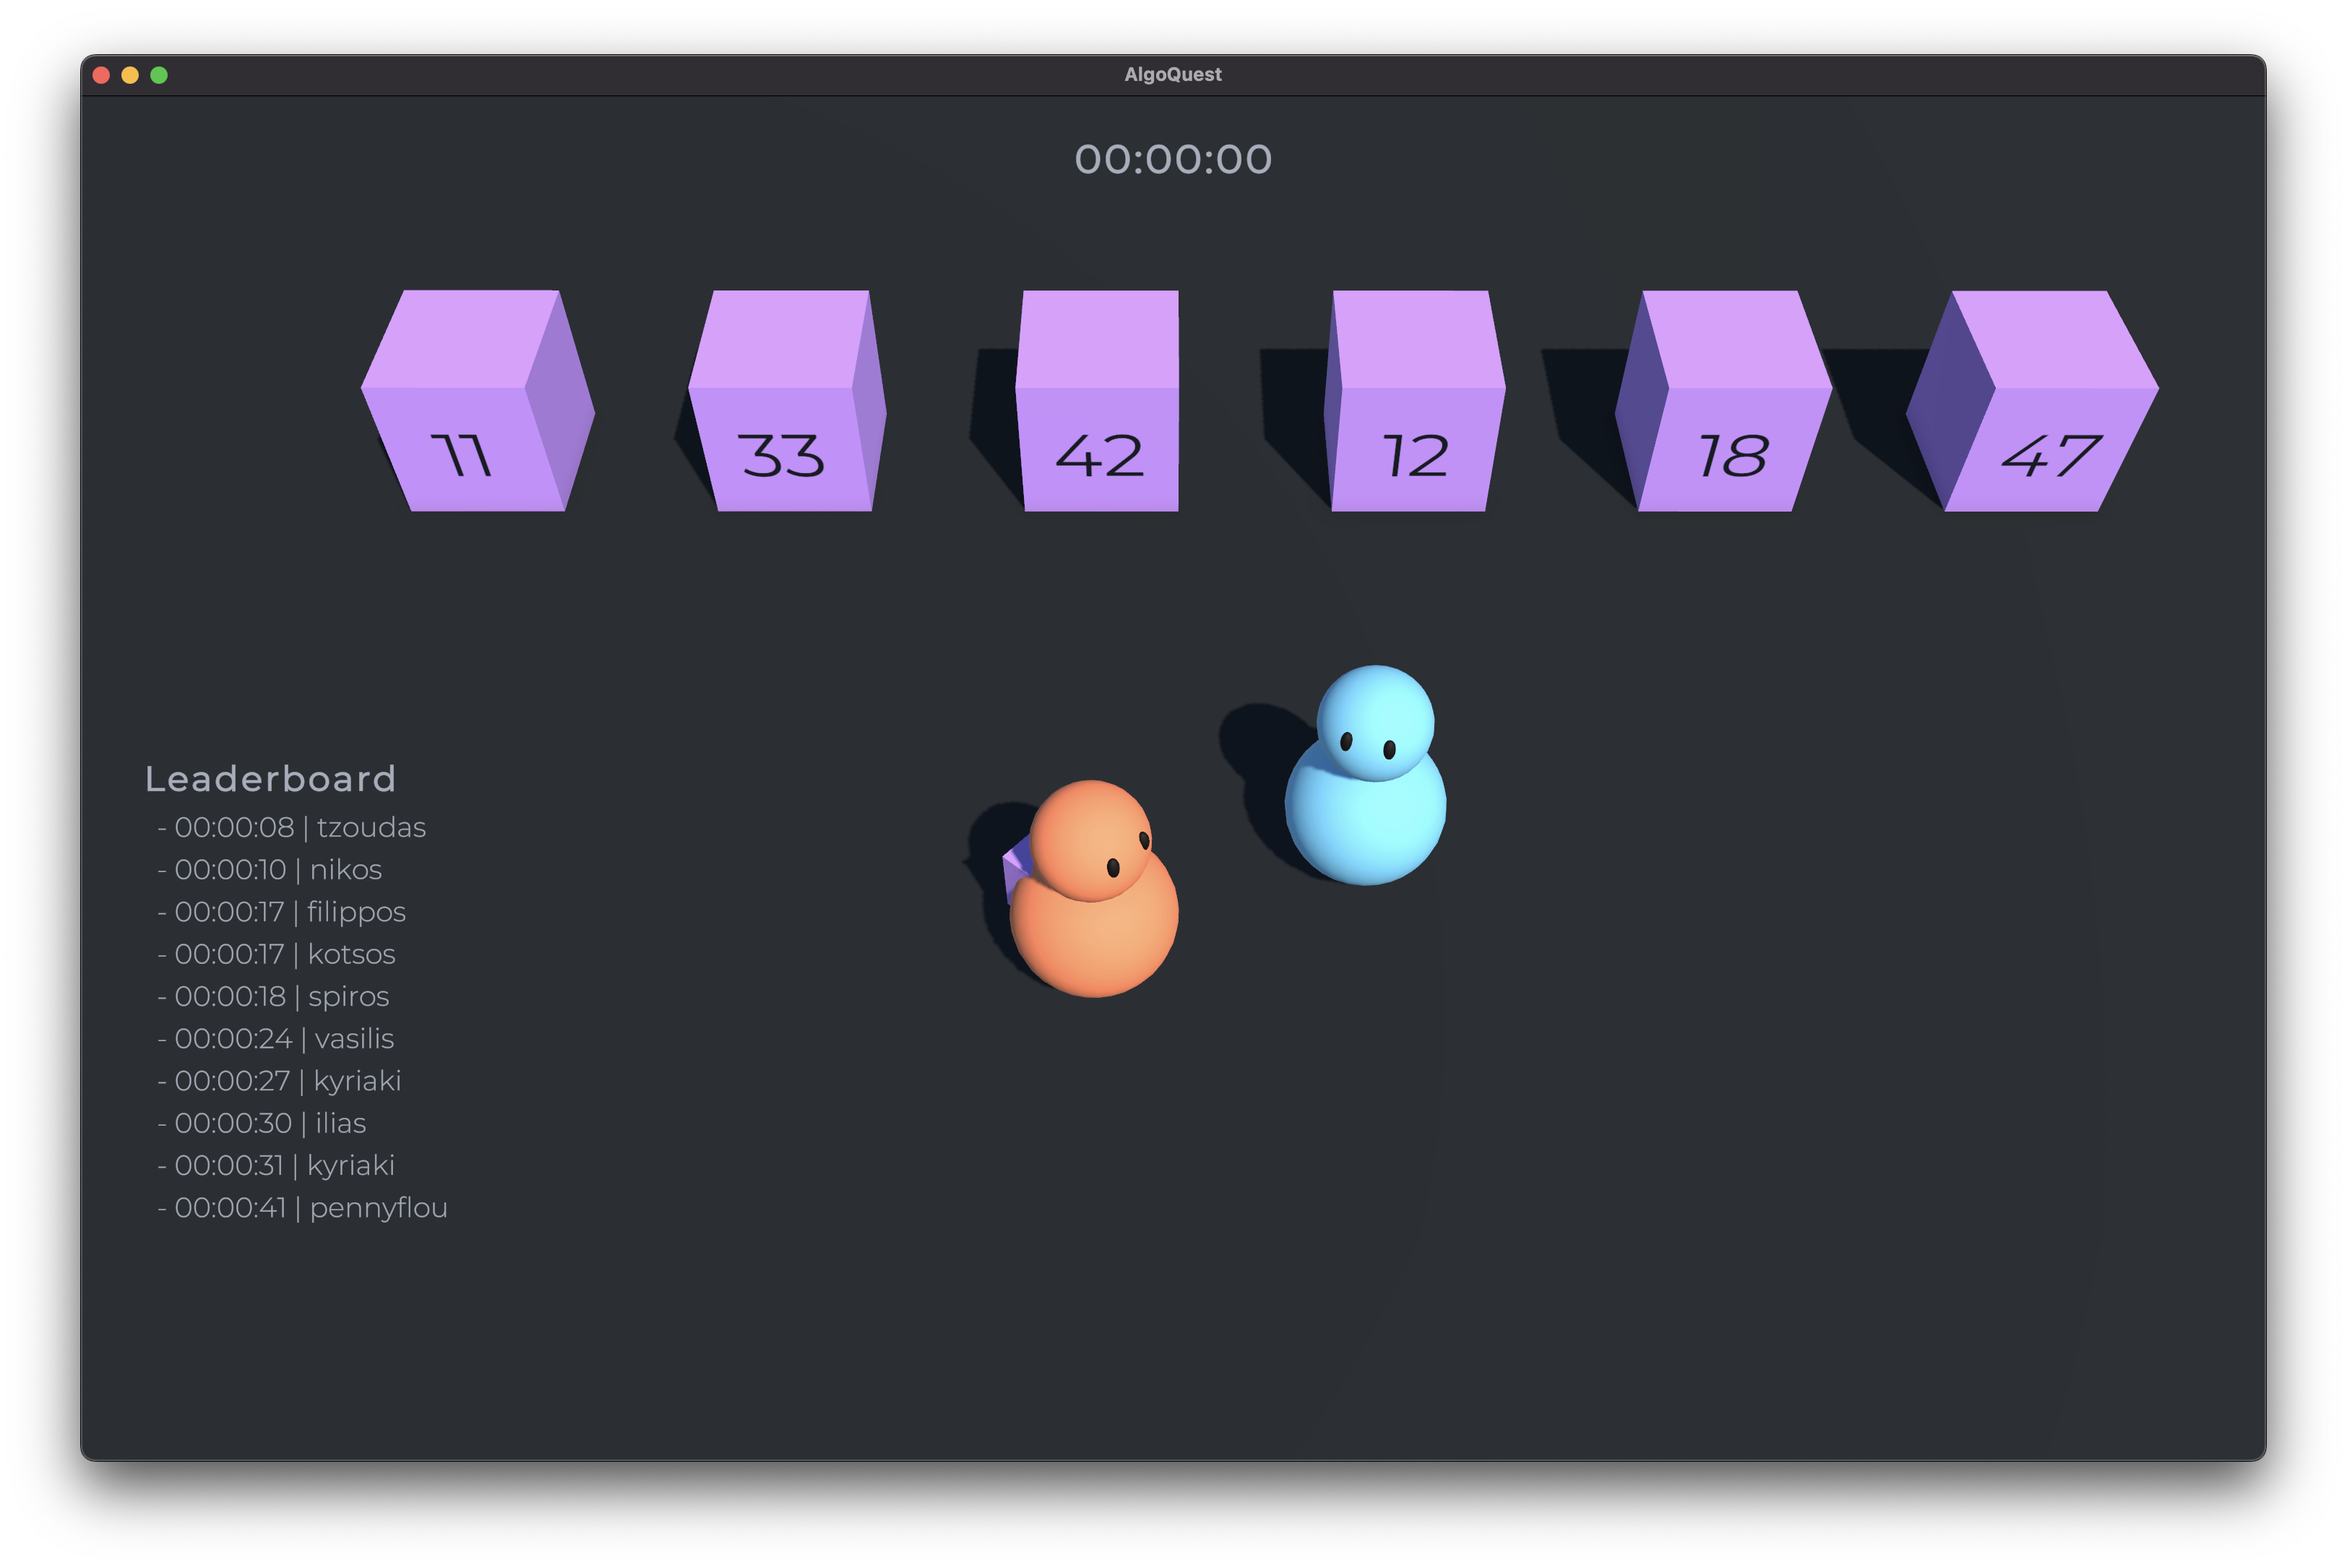
\includegraphics[width=0.8\linewidth]{sections/4/4/images/game_multiplayer}
    \caption{Οι δύο παίκτες στο παιχνίδι}
    \label{fig:game_multiplayer}
\end{figure}

Οι παίκτες διατηρούν τη συμπεριφορά που έχουν όταν είναι και μόνοι τους, και μπορούν να πάρουν, να αφήσουν ή να αλλάξουν τιμές με τα κουτιά. Δεν υπάρχει κάποια αλληλεπίδραση μεταξύ τιμών που μεταφέρουν οι παίκτες, δηλαδή εάν ο παίκτης πάρει μία τιμή από ένα κουτί, ο άλλος δεν μπορεί να αλληλεπιδράσει με αυτή την τιμή πια, μέχρι ο προηγούμενος να την αφήσει.

% ========================================

\subsubsection{Υπηρεσίες}

Η συμμετοχή πολλών παικτών σε ένα κόσμο Unity, μπορεί να γίνει με τη χρήση υπηρεσιών που προσφέρει το Unity, κάτι το οποίο γλιτώνει κάποιον από την υλοποίηση υπηρεσιών για τον σκοπό αυτό. Οι επιλογές που υπάρχουν είναι το \textbf{Unity Relay} και το \textbf{Unity Lobby}, δύο υπηρεσίες που στόχος τους είναι να διευκολύνουν την υλοποίηση ενός κόσμου για πολλούς παίκτες. Και οι δύο επιλογές αυτές κάνουν χρήση του Unity Cloud, μιας υπηρεσίας που προσφέρει το Unity με λειτουργίες και εργαλεία για υλοποίηση παιχνιδιών στο διαδίκτυο.

Το \textbf{Unity Lobby} βασίζεται γύρω από τη δημιουργία λόμπι παικτών πριν μπουν στο παιχνίδι. Ένας παίκτης μπορεί είτε να δημιουργήσει ένα λόμπι στο οποίο μπαίνουν άλλοι παίκτες, είτε να μπει σε λόμπι κάποιου άλλου παίκτη. Αυτό γίνεται είτε μέσω μοναδικού κωδικού που μοιράζεται ο δημιουργός του λόμπι, εφόσον το λόμπι είναι ιδιωτικό, είτε μέσω δημόσιας λίστας, εφόσον ο δημιουργός του λόμπι έχει επιλέξει να το κάνει δημόσιο. Το Lobby έχει την ιδιαιτερότητα πως κάθε λόμπι έχει αποκλειστικό διακομιστή ο οποίος σερβίρει πληροφορίες και δεδομένα σε όλους τους παίκτες\cite{code_monkey_making_2022}.

\begin{figure}[H]
    \centering
    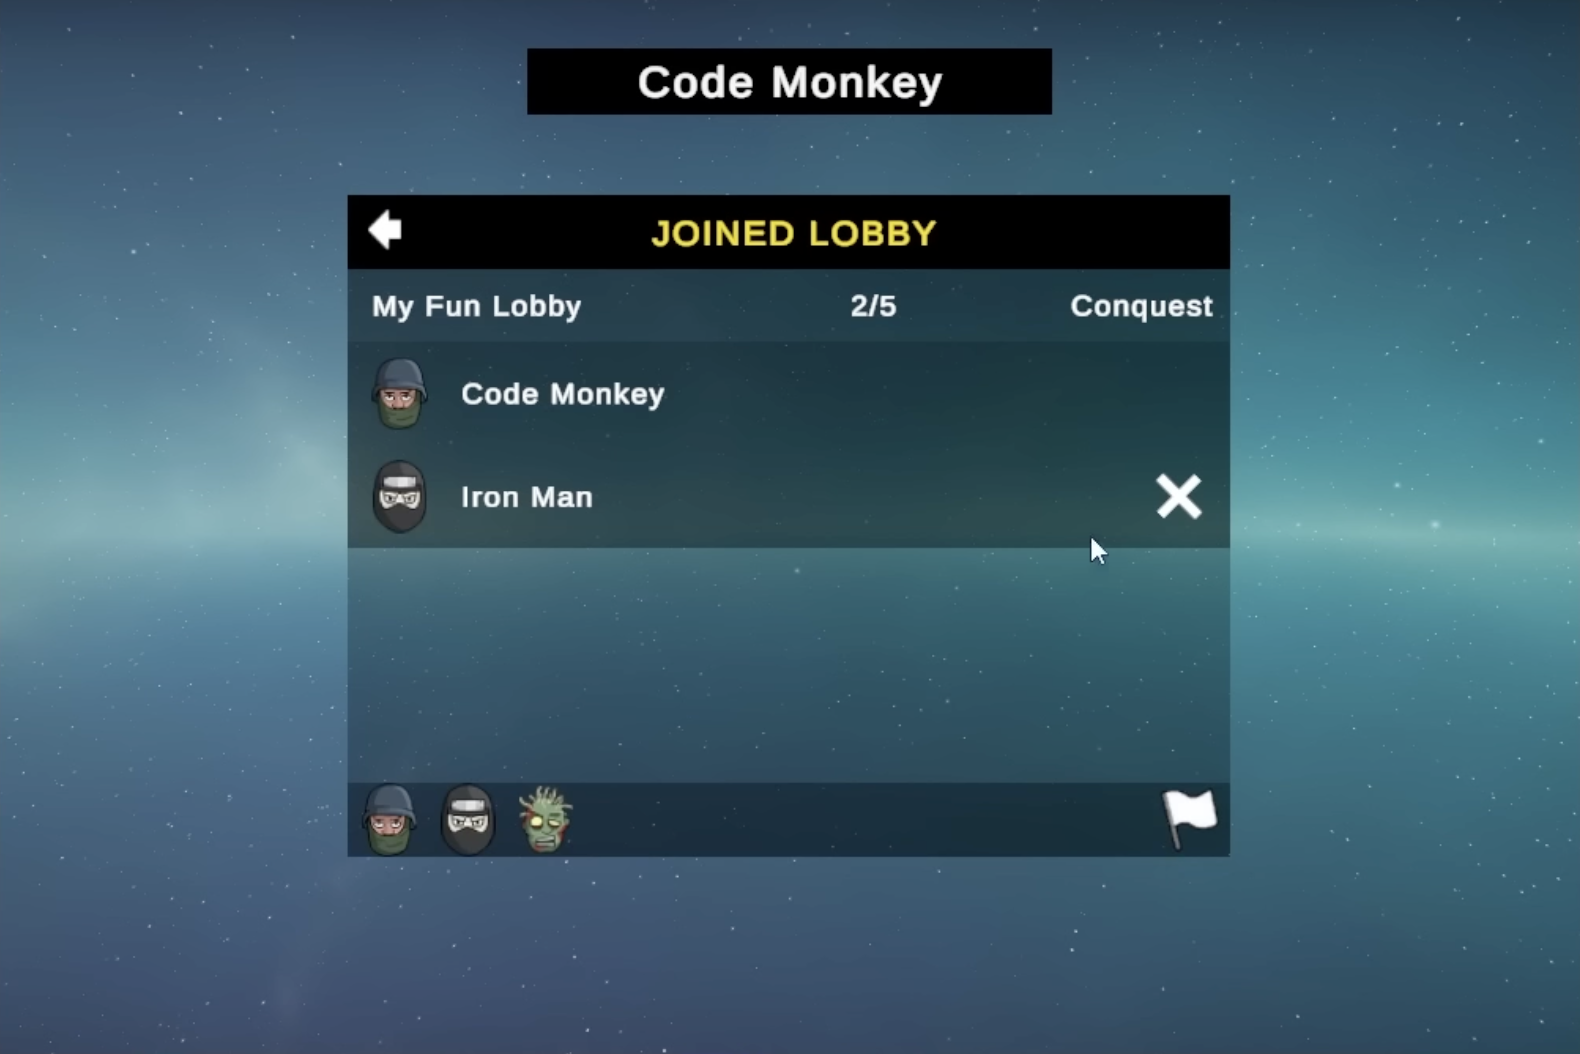
\includegraphics[width=0.8\linewidth]{sections/4/4/images/unity_lobby}
    \caption{Ένα λόμπι με πολλούς παίκτες με χρήση του Unity Lobby}
    \label{fig:unity_lobby}
\end{figure}

Το \textbf{Unity Relay}, σε αντίθεση με το Lobby δεν δημιουργεί τις πληροφορίες για το παιχνίδι και τους παίκτες πριν μπουν στον κόσμο. Αντιθέτως, ένας παίκτης έχει έλεγχο του κόσμου και δημιουργεί έναν διακομιστή στον οποίο μπορούν να συνδεθούν και άλλοι παίκτες ανά πάσα στιγμή, ακόμη και κατά τη διάρκεια του παιχνιδιού. Αυτό σαφώς έχει μεγαλύτερη δυσκολία στην υλοποίηση του κόσμου και της συμπεριφοράς, αλλά προσφέρει μία ροή η οποία συμπληρώνει το γρήγορο ρυθμό του παιχνιδιού πολύ ωραία. Ο τρόπος με τον οποίο συνδέεται ένας παίκτης σε κόσμο που έχει δημιουργήσει ένας άλλος είναι με χρήση μοναδικού κωδικού, στον οποίο έχει πρόσβαση μόνο κάποιος που έχει συνδεθεί στο κόσμο.

\begin{figure}[H]
    \centering
    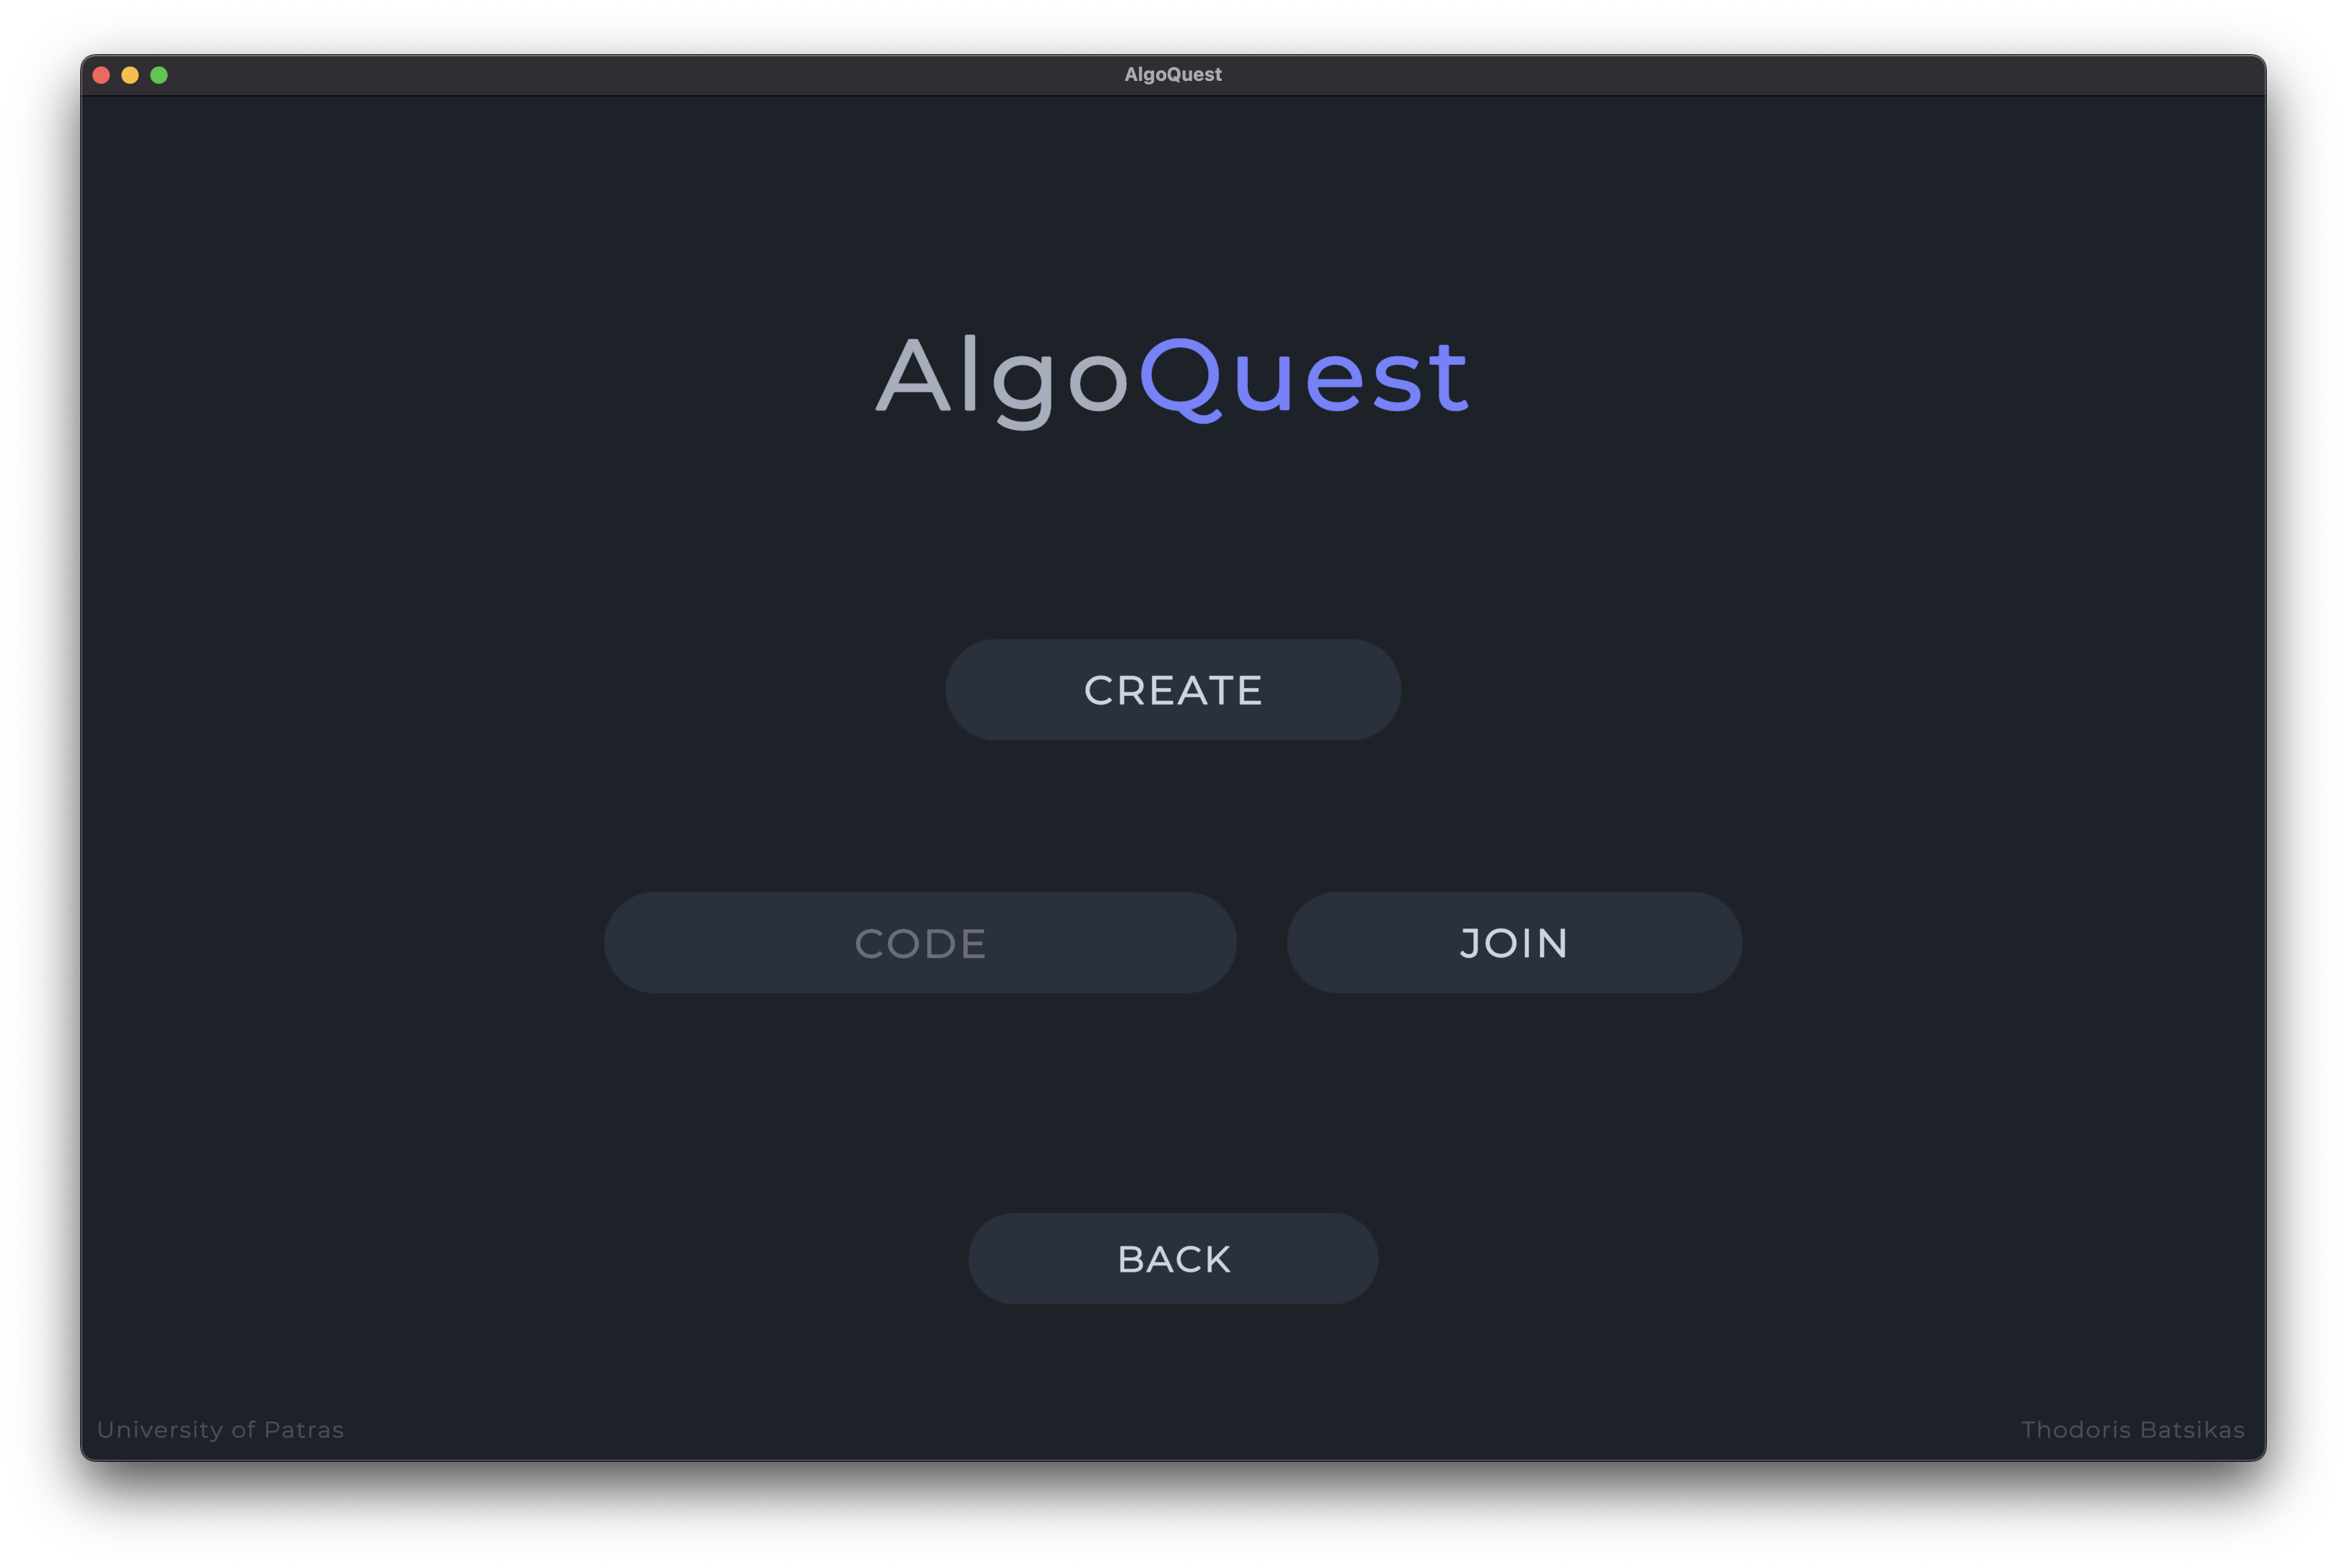
\includegraphics[width=0.8\linewidth]{sections/4/4/images/game_create_or_join_game_menu}
    \caption{Το μενού δημιουργίας ή σύνδεσης στο παιχνίδι με χρήση του Unity Relay}
    \label{fig:game_create_or_join_game_menu}
\end{figure}

\begin{figure}[H]
    \centering
    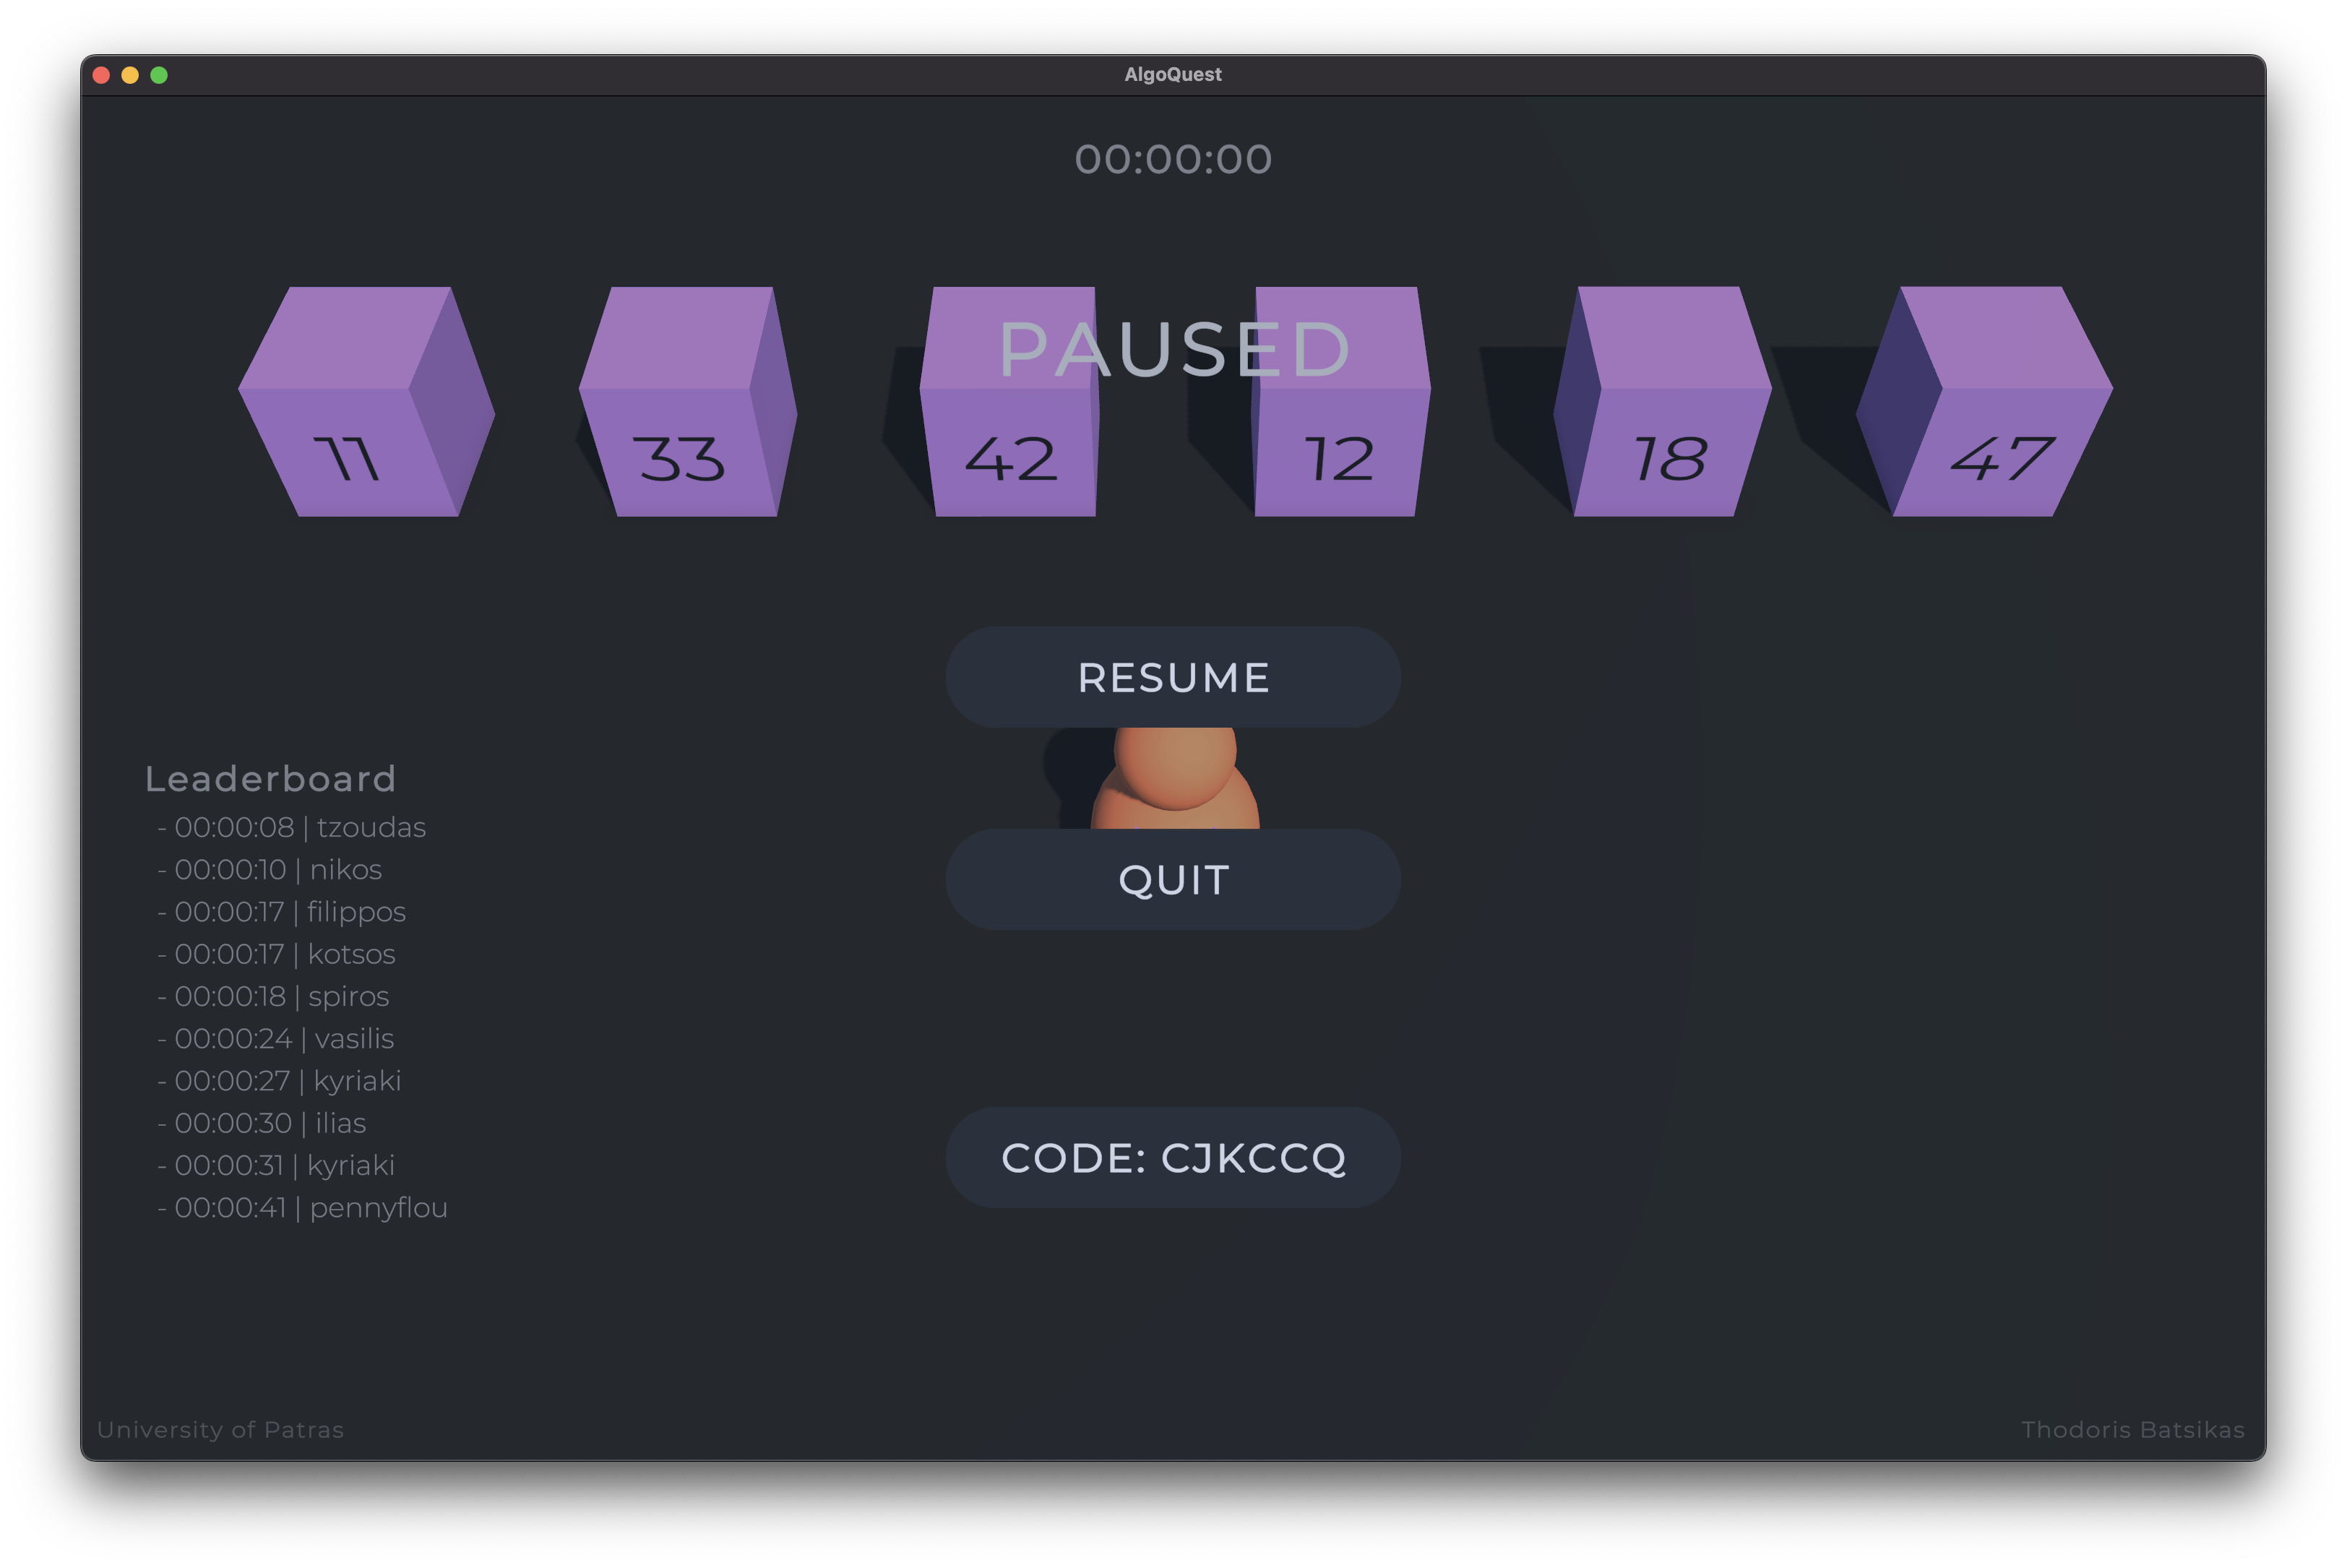
\includegraphics[width=0.8\linewidth]{sections/4/4/images/game_pause_menu}
    \caption{Ο μοναδικός κωδικός που χρησιμοποιείται για τη σύνδεση στον κόσμο στο μενού παύσης του παιχνιδιού}
    \label{fig:game_pause_menu}
\end{figure}

Και στις δύο περιπτώσεις υπάρχει η επιλογή να χρησιμοποιηθεί αποκλειστικός διακομιστής ο οποίος θα σερβίρει όλους του παίκτες, αντί ο αρχικός παίκτης να το κάνει από τον δικό του υπολογιστή. Στη περίπτωση του παιχνιδιού αυτού προτιμήθηκε ο κάθε παίκτης να έχει τον έλεγχο του δικού του κόσμου για ευκολία και απλοποίηση των υποστηρικτικών συστημάτων.

Οι χρήστες ενός παιχνιδιού μέσω διαδικτύου στο Unity είτε μέσω Relay είτε μέσω Lobby, χωρίζονται σε \textbf{\Gls{unity_client}}, που είναι οι χρήστες που δεν τους ανήκει ο διακομιστής, \textbf{\Gls{unity_host}}, που είναι ο ιδιοκτήτης του διακομιστή, και \textbf{\Gls{unity_server}} που είναι ο διακομιστής. Στη περίπτωση αυτή, που δεν υπάρχει αποκλειστικός διακομιστής, ο \Gls{unity_host} και ο \Gls{unity_server} συμπίπτουν.

% ========================================

\subsubsection{Εξουσιοδότηση}

Για να μπορεί ένα παιχνίδι μεταξύ παικτών να λειτουργεί, χρειάζεται δεδομένα τα οποία είναι κοινά για όλους. Δεδομένα όπως η θέση ενός παίκτη ή η τιμή ενός κουτιού είναι όλα πληροφορίες που χρειάζεται να μπορούν να διαβάσουν όλοι οι παίκτες. Το πρόβλημα όμως δημιουργείται όταν οι παίκτες χρειάζεται να γράψουν σε αυτές τις μεταβλητές.

Η δυνατότητα να μπορεί κάποιος να αλλάξει και να γράψει πληροφορίες σε άλλον υπολογιστή μέσω του διαδικτύου αποτελεί μια επικίνδυνη διαδικασία, η οποία είναι ένας παιδότοπος για άτομα με κακή βούληση όπως χακερς. Για την αντιμετώπιση αυτού του προβλήματος, το Unity προσφέρει διάφορες μεθόδους που μπορούν να βοηθήσουν στην αποτροπή αυτών των ατόμων.

Αρχικά, για να μπορεί κανείς να χρησιμοποιήσει τις υπηρεσίες Unity Cloud (π.χ. Unity Relay) χρειάζεται να πιστοποιηθεί πως είναι όντως χρήστης κάποιας εφαρμογής Unity. Στη περίπτωση αυτή γίνεται μέσω script και με τη χρήση της υπηρεσίας \textbf{Unity Authentication}, όπου κάθε παίκτης που επιθυμεί να συνδεθεί σε κάποιο παιχνίδι, περνάει πρώτα από μία ροη πιστοποίησης.

\begin{figure}[H]
    \centering
    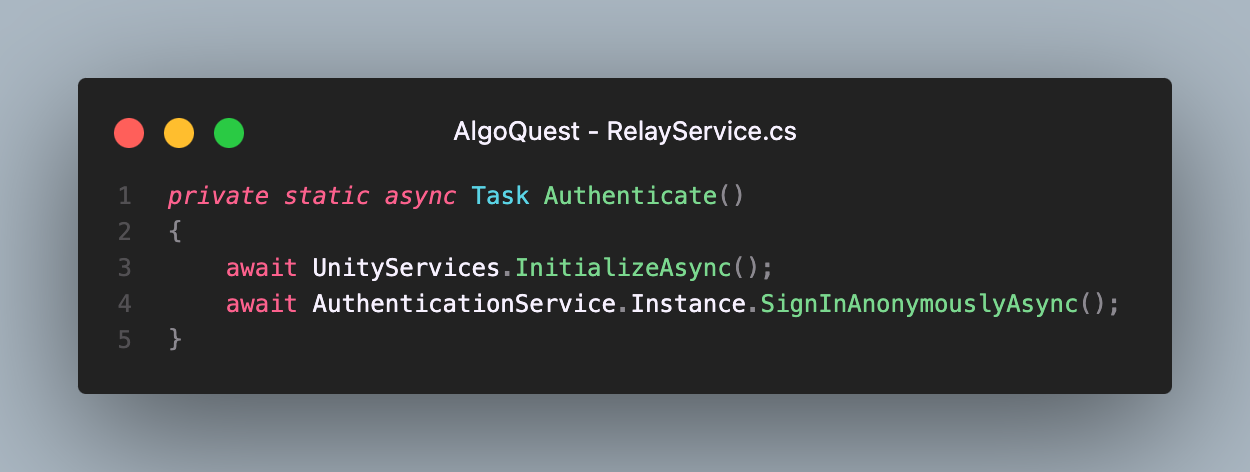
\includegraphics[width=0.8\linewidth]{sections/4/4/images/unity_code_unity_services_auth}
    \caption{Κώδικας που πιστοποιεί ανώνυμα τον παίκτη μέσω της υπηρεσίας Unity Authentication}
    \label{fig:unity_code_unity_services_auth}
\end{figure}

Όσον αφορά την εγγραφή και ενημέρωση δεδομένων από τους \Glspl{unity_client}, μπορούν να εφαρμοστούν δύο τακτικές για την ασφάλεια δεδομένων.

Η πρώτη ονομάζεται \textbf{Client Authoritative} και αναφέρεται στην τακτική όπου ο \Gls{unity_server} δέχεται ότι του στέλνει ένας \Gls{unity_client} χωρίς να ελέγχει κάτι. Αυτό σαφώς δεν είναι πολύ ασφαλές και μπορεί εύκολα να χρησιμοποιηθεί από κακόβουλους χρήστες. Μπορεί για παράδειγμα ένας παίκτης να στείλει πως η θέση του είναι διαφορετική από αυτή που πραγματικά είναι, και επειδή ο \Gls{unity_server} δεν ελέγχει αυτό το μήνυμα, ο χρήστης μπορεί να τηλεμεταφέρεται μέσα στο παιχνίδι. Αυτό σαφώς είναι κάτι μη θεμιτό σε ένα ανταγωνιστικό παιχνίδι. Στη περίπτωση αυτή όμως, η εξαπάτηση του συστήματος δεν έχει σοβαρές επιπτώσεις στα συστήματα του παιχνιδιού, οπότε και έγινε η επιλογή να χρησιμοποιηθεί αυτή η τακτική καθώς είναι πιο εύκολη στην υλοποίηση της.

\begin{figure}[H]
    \centering
    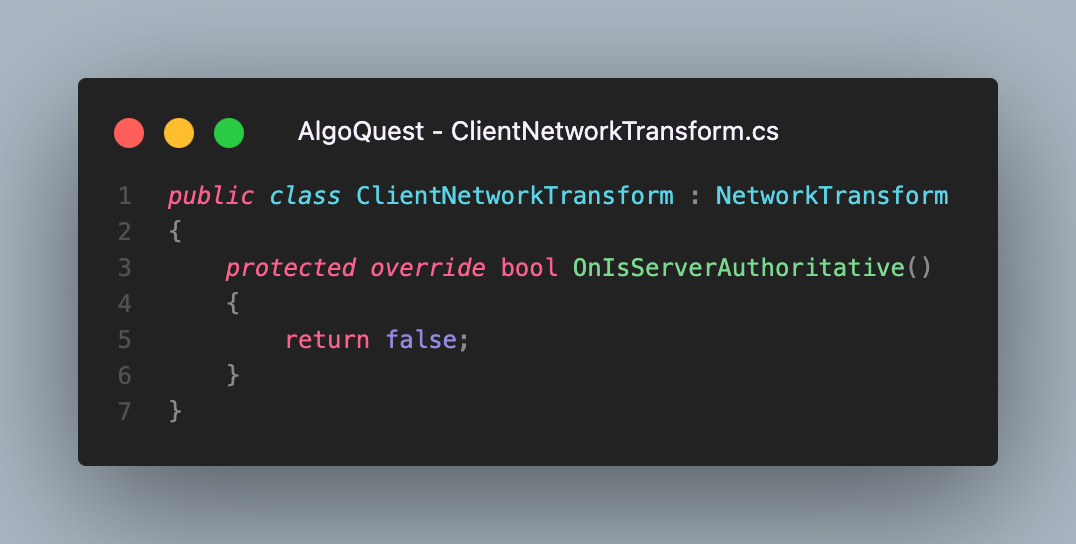
\includegraphics[width=0.8\linewidth]{sections/4/4/images/unity_code_client_network_transform}
    \caption{Κώδικας που επιτρέπει τη μή-ελεγχόμενη αποστολή της θέσης του παίκτη στο \Gls{unity_server}}
    \label{fig:unity_code_client_network_transform}
\end{figure}

Η δεύτερη τακτική ονομάζεται \textbf{Server Authoritative} και είναι η πιο συνηθισμένη σε παιχνίδια \gls{multiplayer}. Σε αντιθεση με την Client Authoritative, εδώ κάθε ενημέρωση δεδομένων γίνεται μέσω του \Gls{unity_server}. Ένας \Gls{unity_client} χρειάζεται να στείλει αίτημα στο Server με τα δεδομένα που θέλει να αλλάξει και ο \Gls{unity_server} ελέγχει αυτό το αίτημα και είτε το εκτελεί είτε το απορρίπτει εφόσον αποφασίσει για την εγκυρότητα του. Η τακτική αυτή είναι σαφώς πιο ασφαλής από την προηγούμενη, αλλά έχει και επιβάρυνση πολυπλοκότητας.

% ========================================

\subsubsection{Κοινόχρηστα δεδομένα}

Σε αντίθεση με ένα απλό παιχνίδι ενός παίκτη, ένα παιχνίδι \gls{multiplayer} ακολουθεί διαφορετικό τρόπο σκέψης και υλοποίησης. Τα δεδομένα που χρειάζεται για να λειτουργήσει είναι της τάξης των gigabyte, γεγονός που καθιστά την μοίραση τους μέσω του διαδικτύου αδύνατη.

Η τεχνική η οποία χρησιμοποιείται λοιπόν είναι η εξής: ο κάθε παίκτης έχει τα δικά του στοιχεία και αντικείμενα και δεδομένα, και μέσω του διαδικτύου μοιράζονται μόνο όσα δεδομένα χρειάζονται. Για παράδειγμα, αντί να μοιράζονται τα μοντέλα των παικτών, ο κάθε παίκτης δημιουργεί τα μοντέλα στον υπολογιστή του, και μέσω διαδικτύου μοιράζεται μονάχα η τοποθεσία τους. Οι τρόποι με τους οποίους αυτά τα δεδομένα μοιράζονται μέσω του διαδικτύου είναι είτε με τη χρήση Network Variables, είτε με τη χρήση \acrshort{rpc}s.

Οι μεταβλητές δικτύου (Network Variables) είναι, όπως υποδηλώνει το όνομα, μεταβλητές δεδομένων που μοιράζονται μέσω διαδικτύου και είναι κοινές για όλους τους παίκτες.

\begin{figure}[H]
    \centering
    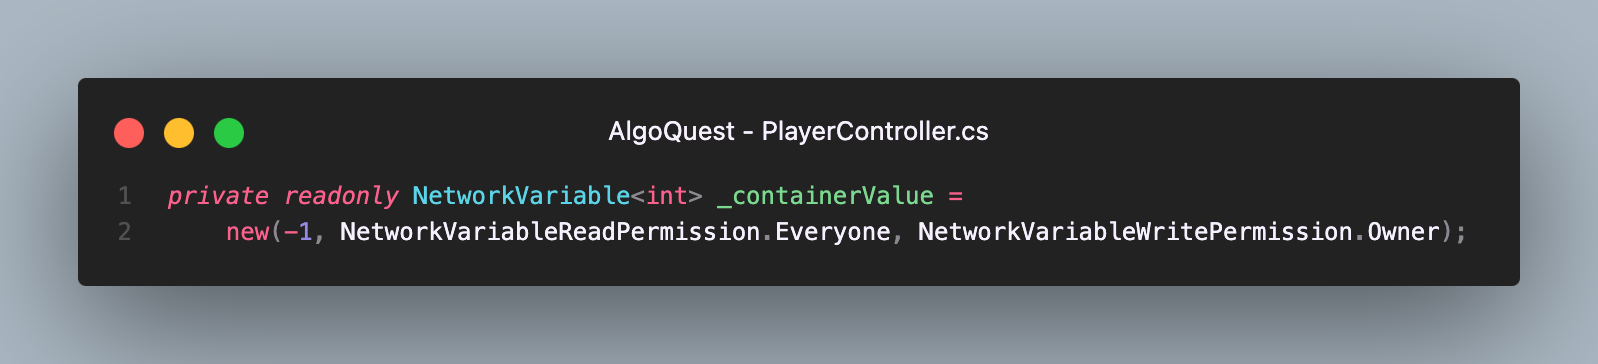
\includegraphics[width=0.8\linewidth]{sections/4/4/images/unity_code_network_variable}
    \caption{Απόσπασμα κώδικα που δημιουργεί μία μεταβλητή δικτύου}
    \label{fig:unity_code_network_variable}
\end{figure}

Οι τύποι αυτών των μεταβλητών μπορεί να είναι οι εξής:
\begin{itemize}
    \item Πρωτόγονοι τύποι C\# (\verb|bool|, \verb|byte|, \verb|int|, \verb|float|, κ.α.)
    \item Ενσωματωμένοι τύποι του Unity (\verb|Vector2|, \verb|Vector3|, \verb|Color|, κ.α.)
    \item Συμβολοσειρές σταθερού μήκους (\verb|FixedString4096Bytes|, κ.α.)
    \item Μεταβλητές που υλοποιούν τη διεπαφή \verb|INetworkSerializable|\cite{noauthor_networkvariables_2024}
\end{itemize}

Αυτές οι μεταβλητές έχουν επίσης ρυθμίσεις για ποιοί χρήστες μπορούν να τις διαβάσουν και να τις ενημερώσουν, κάτι το οποίο προσφέρει ασφάλεια στα δεδομένα που αποθηκεύουν. Δικαίωμα εγγραφής σε Network Variables δεν έχουν οι \Glspl{unity_client}, αλλά μόνο ο ιδιοκτήτης αυτής της μεταβλητής, ή ο \Gls{unity_server}.

Μπορούν να διαβαστούν όπως κάθε άλλη μεταβλητή, αλλά προσφέρουν και events στα οποία μπορεί κάποιος να εγγραφεί και να “ακούει” για αλλαγές όπως το \verb|OnValueChanged|, το οποίο καλείται όταν η μεταβλητή αλλάζει στον \Gls{unity_server}.

\acrfull{rpc} είναι συναρτήσεις που καλούνται σε συγκεκριμένες ομάδες χρηστών που είναι προκαθορισμένες. Αυτές οι συναρτήσεις μπορούν να κληθούν από όλους τους χρήστες, είτε \Glspl{unity_client} είτε \Gls{unity_server}, αλλά εκτελούνται μόνο στις προκαθορισμένες ομάδες\cite{noauthor_rpc_2024}.

Για παράδειγμα ένα \acrshort{rpc} που εκτελείται στον \Gls{unity_server} μπορεί να κληθεί από τους \Glspl{unity_client} με σκοπό την ενημέρωση δεδομένων η οποία θα συμβεί στον \Gls{unity_server}. Με τη σειρά του o \Gls{unity_server}, μόλις κάνει την αλλαγή μπορεί να καλέσει ένα \acrshort{rpc} που εκτελείται σε όλους τους \Glspl{unity_client} με τα νέα δεδομένα. Αυτό το μοτίβο χρησιμοποιείται αρκετά συχνά και αποτελεί τον βασικότερο τρόπο διαχείρισης δεδομένων μεταξύ \Gls{unity_server} και \Gls{unity_client}.

\begin{figure}[H]
    \centering
    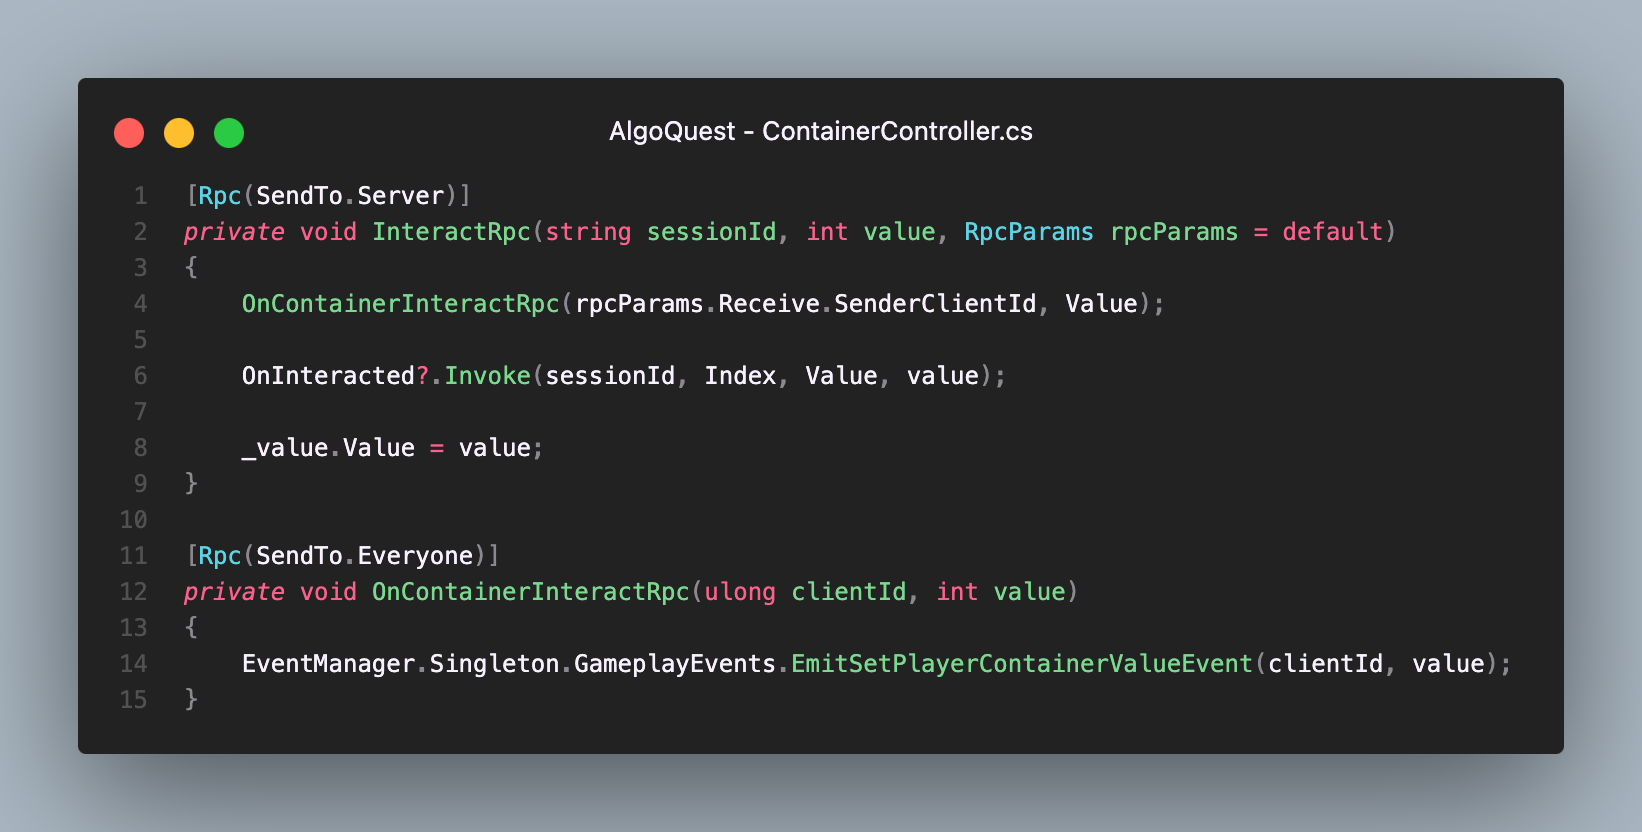
\includegraphics[width=0.8\linewidth]{sections/4/4/images/unity_code_rpcs}
    \caption{Απόσπασμα κώδικα με συναρτήσεις \acrshort{rpc} που εκτελούνται μόνο στον \Gls{unity_server}(επάνω) και σε όλους τους παίκτες(κάτω)}
    \label{fig:unity_code_rpcs}
\end{figure}

% ========================================

\subsubsection{Διάγραμμα ακολουθίας σύνδεσης παίκτη}

\begin{figure}[H]
    \centering
    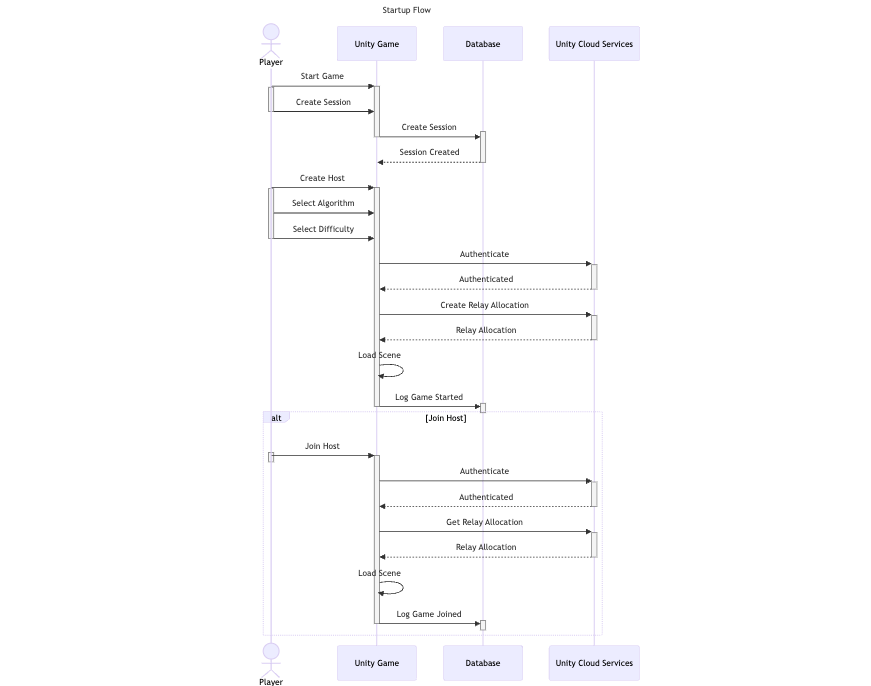
\includegraphics[width=1\linewidth]{sections/4/4/images/startup_flow_sequence_diagram}
    \caption{Διάγραμμα ακολουθίας σύνδεσης παικτών}
    \label{fig:startup_flow_sequence_diagram}
\end{figure}

Για τη δημιουργία του διαγράμματος \ref{fig:startup_flow_sequence_diagram} χρησιμοποιήθηκε το \textbf{Mermaid}\cite{noauthor_mermaid_nodate}.
